\documentclass[11pt]{article}
\usepackage[top=1.6cm,bottom=1.4cm,left=2.5cm,right=2.5cm]{geometry}
\usepackage[T1]{fontenc}
\usepackage{lmodern}
\usepackage{microtype}
\usepackage{parskip}
\setlength{\parskip}{0.65em}
\usepackage{graphicx}
\usepackage{xcolor}
\usepackage[colorlinks=true,allcolors=blue!45!black]{hyperref}
\pagestyle{empty}

\begin{document}

\noindent\today

\medskip
\noindent To the Editors of \emph{Physical Review Letters},

\medskip
\noindent We are pleased to submit our manuscript, \textbf{``A temporally-constrained latent space reveals the stochastic dynamics of convective organization,''} by Sophie Abramian, Olivier Pauluis, L. Ruby Leung, and Pierre Gentine, for consideration as a Letter.

Many systems are high-dimensional and stochastic: identical initial conditions can lead to very different trajectories, in a state space too large to represent directly. How can such systems be reduced to a few variables without losing the dynamics that generate this diversity? We introduce a dimensionality-reduction principle in which the latent representation is constrained to be Markovian. Unlike conventional latent spaces, which preserve geometry, ours preserves the stochastic dynamics themselves: the few retained variables are sufficient to predict their own evolution. %In practice, we train a variational autoencoder coupled with a learned Markov process, building on data-driven Koopman methods and extending them from deterministic to \emph{stochastic} dynamics.

We apply this to atmospheric deep convection, where understanding the origin of intrinsic variability remains a long-standing open problem and a major source of uncertainty in climate projections. We perform cloud-resolving simulations of squall lines (intense, organized storm systems), which exhibit widely different evolutions despite identical large-scale forcing. The method identifies five interpretable states and the Markov transition matrix connecting them. A spectral analysis of this matrix reduces the life cycle of convection to a nearly memoryless walk governed by a single slow mode, from which two competing routes emerge out of a shared suppressed background: a direct ascent into deep organized convection, and a slower drift through weakly organized phases.

A Markovianity assessment shows the description to be nearly, but not exactly, memoryless, and the small departure is itself informative: it indicates what the five states omit. We trace part of this residual memory to cold pools, the cold air left beneath storms. The internal variability of convection is therefore not noise, but a low-dimensional stochastic process between a few physical states, with the residual memory carried by an identifiable physical process.

The principle is general: a reduction constrained by time gives access to the internal variability of a system, the diversity of outcomes it can produce under fixed external conditions, rather than to its mean behaviour alone. We believe the work is well suited to \emph{PRL}.

The manuscript is not published or under consideration elsewhere, and all authors approve this submission.

\smallskip
{\sloppy
\noindent\textbf{Suggested reviewers:}
Elizabeth Barnes, Colorado State University (eabarnes@colostate.edu);
Zhiming Kuang, Harvard University (kuang@fas.harvard.edu);
Allison Wing, Florida State University (awing@fsu.edu);
Cathy Hohenegger, MPI for Meteorology (cathy.hohenegger@mpimet.mpg.de);
Brian Mapes, University of Miami (bmapes@miami.edu).\par}

\smallskip
\noindent Thank you for considering our manuscript.

\smallskip
\noindent Sincerely,\\[1mm]
\noindent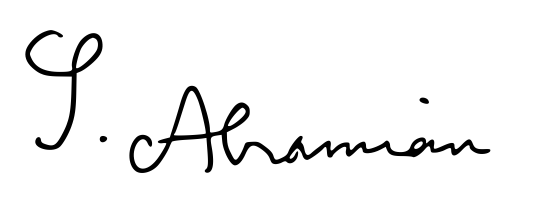
\includegraphics[width=3.2cm]{signature.png}\\[-0.5mm]
{\small
Sophie Abramian, on behalf of the authors\\
Department of Earth and Environmental Engineering, Columbia University\\
\href{mailto:sophie.abramian@gmail.com}{sophie.abramian@gmail.com}
}

\end{document}